\section{Obfuscation evaluations}
\subsection{Evaluations criteria}
Collberg\cite{16} gives an accurate definition on code obfuscation: The i is one of all possible inputting set \emph{I} which is in the program \emph{P}. If and only if it is $\forall$ \emph{i:T(P)(i)=P(i)}, we can just think that the transition of the confusion was correct. The obfuscation method is evaluated from potency, resilience and cost by Collberg at al.

Let \emph{T} be a behavior-conserving transformation, such that \emph{P $\underrightarrow{T}$ P'} transforms a source program \emph{P} into a target program \emph{P'}.

\emph{T$_{pot}$(P)}, the potency of \emph{T} with respect to a program \emph{P}, is a measure of the extent to which \emph{T} changes the complexity of \emph{P}. Let \emph{E(P)} be the complexity of \emph{P}.  It is defined as

 \begin{equation}\emph{T$_{pot}$(P)=E(P')/E(P)-1}\end{equation}

 \noindent T is a potent obfuscating transformation if \emph{T$_{pot}$(P)>0}.

\emph{T$_{res}$(P)} is the resilience of \emph{T} with respect to a program \emph{P}. \emph{T$_{res}$(P)=one-way} if information is removed from \emph{P} such that \emph{P} cannot be reconstructed from \emph{P'}. Otherwise,

 \begin{equation}\emph{T$_{res}$(P)$\triangleq$ Resilience(T$_{Deobfuscaor effort}$,T$_{Programmer effort}$)}\end{equation}

\emph{T$_{cost}$(P)} is the extra execution time/space of \emph{P'} compared to \emph{P}. that is to say

\begin{equation}\emph{T$_{cost}$(P)=Cost(C$_{time}$ , C$_{size}$)}\end{equation}

\subsection{Evaluations based on smali code obfuscation}
Potency. The proposed code confusion method includes both control obfuscation and data obfuscation. In data obfuscation, we can obfuscate the instructions of accessing the values from the registers and calling method that its returned value is object type. In control obfuscation, in order to resist attacker to accessing the returned values which is after calling the key function, we will insert the opaque predicate between two instructions that are calling and accessing returned value. The above two kinds of method can both resist the attacker to acquire correct program code and increase the complexity of the control flow. Thus, the method of proposed has good strength.

Resilience. The obfuscated program has been analyzed from the point of reverse analysis. For example, the attacker can't accessing correct instructions and analyzing logical construction of program. As shown in Figure~\ref{fig:Figure 7}, decompilation process is failure and control flow becomes very complicated. so the method of proposed has strong slastic.

Cost. The function's time complexity is O(1) after being obfuscated. Firstly, inserting opaque predicate and modifying the instruction format is not to change polynomial of the complexity. Secondly, dex dynamic loading and backfilling the bytecode both increasing little time, but as shown in Figure \ref{fig:Figure 8}, only the first launching time increases more. In space consumed, we will only insert opaque predicate into invoking the key function and obfuscated instructions is short. Thus this method has little effect on the time and space consumed.


\begin{figure}[!tbp]
  \centering
  % Requires \usepackage{graphicx}
  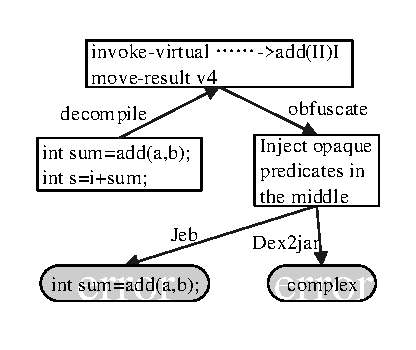
\includegraphics[width=0.8\columnwidth]{fig/fig7.pdf}
  \caption{The case of reversing engineering. When we inject the opaque predicates after invoking the \emph{add()} method, the attacker can't capture the return-value \emph{sum.}}\label{fig:Figure 7}
\end{figure}
\section{Evaluation}

\subsection{Experimental Setup}
\paragraph*{Hardware} Our approach is evaluated using a Huawei Nexus 6p phone, which runs the Android 6.0 Marshmallow operating system. The device has two processors: a four-core ARM Cortex-A57 processor at 1.95 GHz and a four-core ARM Cortex-A53 processor at 1.55 GHz. 
The device has 3 GB of RAM and 64 GB of internal storage. 

\paragraph*{Benchmarks} Our approach is evaluated by using the developed tool to protect a set of representative operations of typical Android applications. We have implemented these operations in four applications (listed Table~\ref{tab:Table 1}).
These test cases represent \FIXME{xx, xx, xx. Explain these operations }. 

%Based on the deep research in SmaliPro, as shown in Fig.2, this paper designed and implemented a prototype system. It can resist the static analysis and dynamic analysis of the process of the reverse engineering. All experiment are conducted on the Android virtual decice of Android Version 4.2, which has 512M RAM, and 256M internal storage.

%To measure the performance overhead and effectiveness of SmaliPro, we first selected four typical applications which have different instructions as test case. These four apps are listed in Table~\ref{tab:Table 1}.

\begin{table}[htbp]
  \centering
  \rowcolors{2}{gray!25}{white}
  \begin{tabular}{c c}
  \toprule
  Test case & The characteristics of the instruction\\
  \hline
  \hline
  Long.apk & Define 32-bits constant\\


  Re\_objapk & Returned value of the reference type\\


  Key\_fuc.apk & key function(self-defined)\\


  Compre.apk & All the above\\
  \bottomrule
  \end{tabular}
  \caption{A list of apps we selected to test. Column 2 represent the type of instructions of four typical Android apps. }\label{tab:Table 1}
  \FIXME{Where did you get these applications?}
\end{table}

\subsection{Effectiveness}
The main purpose of this paper is to protect the executable code of the application, and make it not be easy analyzed by attacker. The below from two aspects of resisting static and dynamic  analysis analyze the effectiveness of the protection method based on confusion of smali code.

The some bytecode within executable file is a zero sequence before executed bytecode flow by DVM. So when attackers want to statically analyze the logical structure of the program, they can't acquire correct bytecode. Before the app running the attackers dump the bytecode through dynamically analyzing, this way is the same with resisting static analysis. If running, they will dump the obfuscated bytecode, which isn't correctly decompiled, as shown in Figure~\ref{fig:Figure 5}.

In order to the effectiveness of the obfuscated method, we will also utilize reversing tools to reverse executable code of the application. The experiment results is shown in Table~\ref{tab:Table 2}.

\begin{table}[htbp]
  \centering
  \rowcolors{2}{gray!25}{white}
  \begin{tabular}{c c c c c}
  \toprule
  Test case & Jeb & Dex2Jar & dexdump & IDA pro\\
  \hline
  \hline

  Long.apk  & $\times$ & $\times$ & $\ast$ & $\ast$\\


  Re\_objapk & $\times$ & $\times$ & $\ast$ & $\ast$\\


  Key\_fuc.apk & $\times$ & $\ast$ & $\times$ & $\ast$\\


  Compre.apk & $\times$ & $\times$ & $\times$ & $\ast$\\
  \bottomrule
  \end{tabular}
   \caption{The results of analysis by reversing tools. $\times$ represent that the code after reversing is wrong. $\ast$ represent that it becomes very complicated}\label{tab:Table 2}
\end{table}

\subsection{Performance overhead}
We measured the performance overhead of SmaliPro by comparing the executable file size, memory use and launch time of applications before and after obfuscated by SmaliPro.

Table~\ref{tab:Table 3} illustrates the file size and memory use changes of applications before and after obfuscated. we can see that the dex file size increases more than 300 bytes. This increase in file size is mainly due to the packer dex file that is used to load really dex file and inserting the instructions. The results are not obvious because the application size we selected is relatively small and little difference.

We will describe that memory costs are mainly caused by the paker dex file and native library. But current mobile devices tend to provide more RAM, you can ignore the costs.

To measure the app response delay after being protected by SmaliPro, we compared the app launch time for the first, second, third, and fourth run before and after obfuscated. To make it more precisely, we did each experiment 20 times and used the average value as a final reference. The launch time of four test case is listed in Table~\ref{tab:Table 4}.

Figure~\ref{fig:Figure 8} shows the app launch time changers at each time. We can see that the time increase at the first launch, which is mainly caused by: 1) running the obfuscated application needs to replace Classloader; 2) Before running we must find the obfuscated method in the corresponding memory address through parsing the structure of the dex file and then fill the bytecode that is stored in ObjMethod in the address. These classes and libraries will be loaded at the application's first execution and will be kept in the memory so long as the system resources are sufficient. Thus, they do not need to be loaded again in the app's latter launch, which is the reason why they all show a similar launch time as the unprotected apps at the latter launch.

\begin{figure}
  \centering
  % Requires \usepackage{graphicx}
  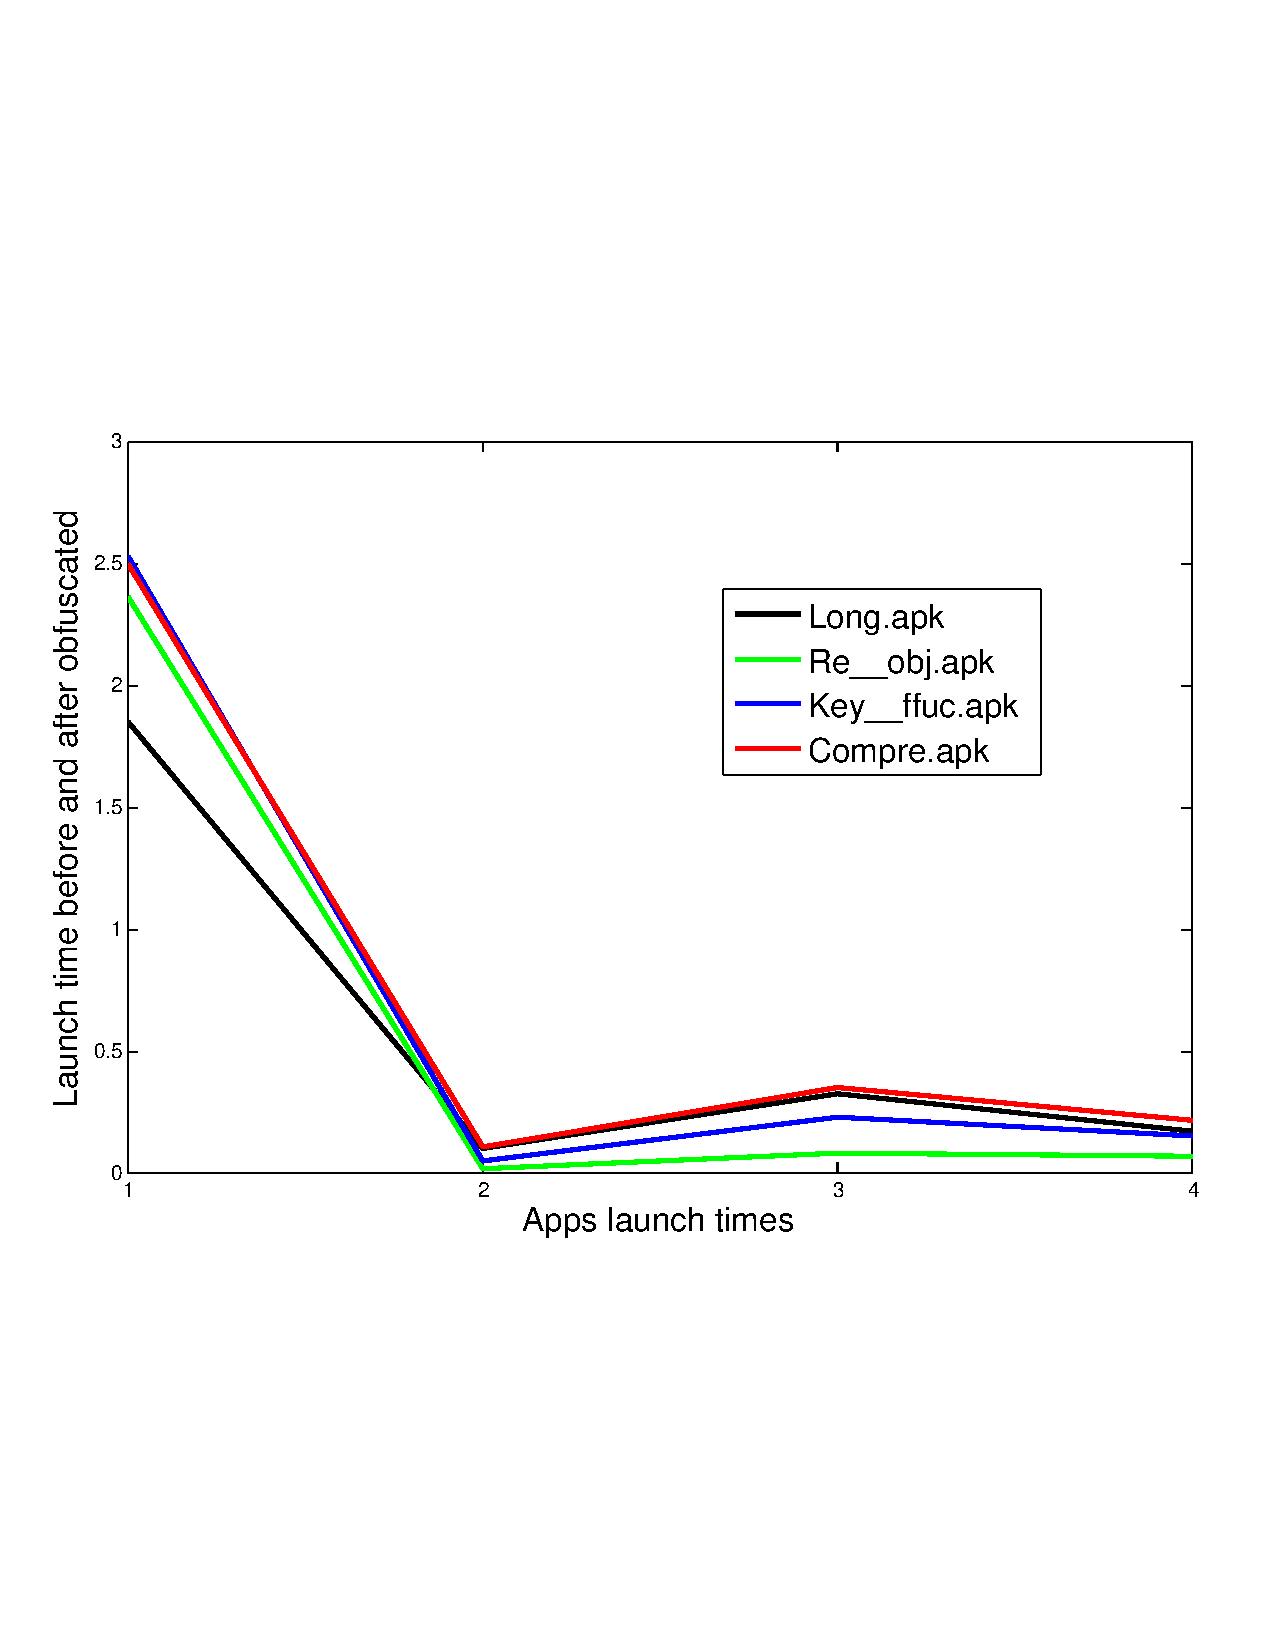
\includegraphics[width=0.8\columnwidth]{fig/fig8.pdf}\\
  \caption{Describe the changes of launch time D-value. Compare to the first ,second, third ,and fourth launch time D-value before and after obfuscated. we can see only that the time significantly increase at the first launch  }\label{fig:Figure 8}
\end{figure}


\begin{table}[htbp]
  \centering
  \begin{tabular}{c c c c c}
  \toprule
  \multirow{2}{*}{Test case} & \multicolumn{2}{c}{Dex file size (bytes)} & \multicolumn{2}{c}{Memory use(KB)}\\
  \cline{2-5}
  \cmidrule{2-5}

  & Before & After &  Before & After\\
  \hline

  Long.apk & 449040 & 462328 & 4320 & 5858\\
   \rowcolor{mygray}


  Re\_obj.apk & 449080 & 462392 & 4072 & 7082\\


  Key\_fuc.apk & 449176 & 462483 & 4349 & 6248\\

\rowcolor{mygray}
  Compre.apk & 449232 & 462556 & 4866 & 6406\\
  \bottomrule
  \end{tabular}
  \caption{Comparison of file size and memory use before and after obfuscated. Column 2 and Column 3 represent the size changes of dex file before and after obfuscated. Column 4 and Column 5 shows the size changes of memory use.}\label{tab:Table 3}
  \FIXME{Show increase code size and memory footprint in percentages in bar charts.}
\end{table}

\begin{table*}[htbp]
  \centering
  \begin{tabular}{c c c c c c}
  \toprule

  \multicolumn{2}{c}{Test case} & Long.apk & Re\_obj.apk & Key\_fuc.apk & Compre.apk\\
  \hline
   \hline
  \multirow{2}{*}{First(s)} & Before & 2.175 & 2.249 & 2.124 & 2.912\\
  & After & 4.027 & 4.612 & 4.677 & 5.412\\
  \hline


  \multirow{2}{*}{Second(s)} & Before & 0.939 & 0.923 & 0.844 & 0.911\\
  & After & 1.027 & 0.942 & 0.892 & 1.017\\
  \hline

  \multirow{2}{*}{Third(s)} & Before & 0.845 & 0.882 & 0.797 & 0.891\\
  & After & 1.171 & 0.959 & 1.024 & 1.238\\
  \hline

  \multirow{2}{*}{Fourth(s)} & Before & 0.823 & 0.862 & 0.781 & 0.887\\
  & After & 0.994 & 0.928 & 0.934 & 1.099\\

  \bottomrule
  \end{tabular}
   \caption{Launch time(in seconds) of four apps for the four times launch before and after obfuscated.}\label{tab:Table 4}
\end{table*} 